% -*- coding: UTF-8 -*-
% hurlex-chapt7.tex
% hurlex 开发文档 第7章内容

\section {添加中断描述符表}

\subsection{中断的引入}

\par 中断是用以提高计算机工作效率、增强计算机功能的一项重要技术。其实简单说中断就是一种通知机制罢了。我们知道操作系统的一个\allowbreak
核心任务就是和连接在主板上的所有的硬件设备进行通信,但是CPU和这些外设的速率根本就不在一个数量级上,倘若CPU向某一个设备发出一\allowbreak
个请求并且一直等待反馈结果的话,这样带来的性能损失是不可接受的。而且CPU在运行期间需要得知外设所发生的事件,轮询显然是不可取\allowbreak
的,那么就迫切需要一种机制来帮助我们解决这个问题。

\par 肩负着这一伟大使命,中断应运而生。当某个中断发生时,典型的处理方式就是CPU会打断当前的任务,保留当前的执行现场后再\allowbreak
转移到该中断事先安排好的中断处理函数\footnote{或者叫中断服务例程。}去执行。在中断处理函数执行结束之后再恢复中断之前的执\allowbreak
行现场,去执行之前的任务。

\par 从物理学的角度看,中断其实就是一种电信号,一般由硬件设备生成并送入中断控制器统一协调\footnote{当然需要一个"协调机构"了,\allowbreak\
试想所有设备不区分轻重缓急的和CPU发送中断信号的恐怖场景…}。中断控制器就是个简单的电子芯片,其作用就是将汇集的多路中断管线,采用\allowbreak
复用技术只通过一条中断线和CPU相连接。既然中断控制器这里只有一条线和CPU相链接,那么为了区分各个设备,中断自然就有编号了。

\par 补充一下,其实CPU的中断管脚并非只有一根,其实是有NMI和INTR两个管脚,因为从严重性上来看,中断是分为两类的,首先NMI管脚触发的\allowbreak
中断是需要无条件立即处理的,这种类型的中断是不会被阻塞和屏蔽的,所以叫做非屏蔽中断(Non Maskable Interrupt, NMI)。\allowbreak
事实上一旦产生了NMI中断,就意味着CPU遇到了不可挽回的错误,一般不会进行处理,只是给出一个错误信息。而我们之前所说的中断\allowbreak
控制器连接的管脚叫做INTR,这类中断有两个特点,分别是数量多和可屏蔽。而我们主要关注的正是INTR中断。

\par 举一个通俗的例子,假设你就是CPU,你正在看书(执行任务),突然间你的鼻涕流下来了(一个NMI中断),这个自然是不可以屏蔽的,\allowbreak
不然会流到嘴里的…(好恶心),你现在把书反着扣在桌子上避免找不到页码(保留当前执行现场),取出纸巾…(此处省略几十个字),OK,\allowbreak
你处理完后把书拿起来继续看(恢复之前的执行现场)。这就是一个中断的处理过程,其实很简单是不是?这是不可屏蔽中断,那么可屏蔽\allowbreak
的呢?还是刚刚那个场景,你在看书,手机响了(一个INTR中断),但是你在学习期间不想被打扰,就无视它了…这就是可屏蔽中断了。

\par 通俗的例子举完了,我们还是专业一点好了。在x86PC中,我们熟知的中断控制芯片就是8259A PIC了,它就是我们说的中断控制器了。Intel的\allowbreak
处理器允许256个中断,中断号范围是0~255。8259A PIC芯片负责15个,但是并不固定中断号,允许通过IO端口设置以避免冲突。它的全称\allowbreak
是可编程中断控制器(Programmable Interrupt Controller,PIC)。关于8259A PIC的资料网上铺天盖地的,至于8259A PIC的结构,\allowbreak
如何屏蔽中断什么的我就不多说了,请大家自行去了解。

\par 其实从上面的描述中我们基本上能理解中断的概念了。再简单说就是硬件发生了某个事件后告诉中断控制器,中断控制器汇报给CPU,\allowbreak
CPU从中断控制器处得知了中断号,根据这个中断号找到对应的中断处理程序并转移过去执行,完成后重新回到之前的执行流程去。

\par 我们之前一直说的都是硬件中断,其实除了硬件中断之外还有软件中断,也就是软件系统也可以利用中断机制来完成一些任务,\allowbreak
比如有些OS的系统调用的实现就采用了中断的方式。

\subsection{中断的实现}

\par 我们的重点是保护模式下的中断处理。中断处理程序是运行在ring0层的,这就意味着中断处理程序拥有着系统的全部权限,仿照内存段\allowbreak
描述符表的思路,Intel设置了一个叫做中断描述符表(IDT, Interrupt Descriptor Table)的东西,和段描述符表一样放置在主存中,\allowbreak
类似地,也有一个中断描述符表寄存器(IDTR)记录这个表的起始地址。那么下文的重点就是这个中断描述符的结构和设置方法了,其实\allowbreak
这里很类似GDT的那一套过程,我们先给出中断描述符表的结构:\allowbreak
\footnote{照例引用Intel文档中的插图,这是一篇开源的文档,应该没有版权纠纷吧...}

\begin{figure}[ht]
      \centering
      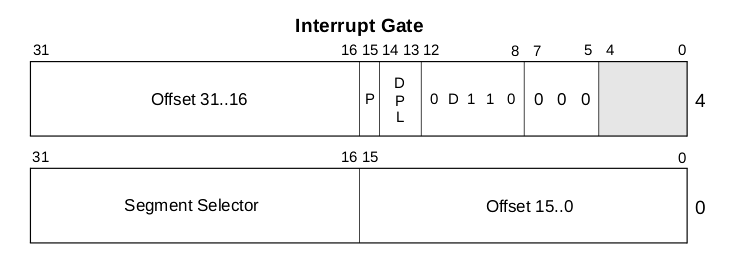
\includegraphics[scale=0.5]{picture/chapt7/interrupt_gate.png}
      \caption{中断描述符的格式}
\end{figure}

\par 根据这个描述信息,我们给出相关的C语言结构体定义:

\begin{lstlisting}[language = C, caption = include/idt.h]
#ifndef INCLUDE_IDT_H_
#define INCLUDE_IDT_H_

#include "types.h"

// 初始化中断描述符表
void init_idt();

// 中断描述符
typedef
struct idt_entry_t {
	uint16_t base_lo;        // 中断处理函数地址 15 ~ 0 位
	uint16_t sel;            // 目标代码段描述符选择子
	uint8_t  always0;        // 置 0 段
	uint8_t  flags;          // 一些标志,文档有解释
	uint16_t base_hi;        // 中断处理函数地址 31 ~ 16 位
}__attribute__((packed)) idt_entry_t;

// IDTR
typedef
struct idt_ptr_t {
	uint16_t limit; 	// 限长
	uint32_t base; 		// 基址
} __attribute__((packed)) idt_ptr_t;

#endif 	// INCLUDE_IDT_H_
\end{lstlisting}

\par 之前我们建立了中断的概念并且介绍了描述符表的结构,接下来我们细化CPU处理中断的\allowbreak
过程,首先是起始过程,也就是从CPU发现中断事件后,打断当前程序或任务的执行,根据某种机制跳转到中断处理函数去执行的过程:
\begin{enumerate}
	\item CPU在执行完当前程序的每一条指令后,都会去确认在执行刚才的指令过程中是否发送中断请求过来,如果有那么CPU\allowbreak
		就会在相应的时钟脉冲到来时从总线上读取中断请求对应的中断向量。然后根据得到的中断向量为索引到IDT中找到该向量\allowbreak
		对应的中断描述符,中断描述符里保存着中断处理函数的段选择子;
	\item CPU使用IDT查到的中断处理函数段选择子从GDT中取得相应的段描述符,段描述符里保存了中断处理函数的段基址和属性信息。\allowbreak
		此时CPU要进行一个很关键的特权检验的过程,这个涉及到CPL、RPL和DPL的数值检验以及判断是否发生用户态到内核态的切换。\allowbreak
		如果发生了切换,还要涉及到TSS段和用户栈和内核栈的切换;\footnote{这些东西我们之前都没有说过,所以大家看不懂的话\allowbreak
		就先跳过去,等到后面讲到保护环的时候我们再细说。}
	\item 确认无误后CPU开始保存当前被打断的程序的现场(即一些寄存器的值),以便于将来恢复被打断的程序继续执行。这需要利用内核栈来保存\allowbreak
		相关现场信息,即依次压入当前被打断程序使用的eflags、cs、eip、以及错误代码号(如果当前中断有错误代码);
	\item 最后CPU会从中断描述符中取出中断处理函数的起始地址并跳转过去执行。
\end{enumerate}

\par 以上是起始过程,中断处理函数执行完成之后需要通过iret或iretd指令恢复被打断的程序的执行。这时候比较简单,首先CPU会从内核栈\allowbreak
里弹出先前保存的被打断的程序的现场信息,即之前的eflags,cs,eip重新开始被打断前的任务。\allowbreak
\footnote{如果之前存在特权级转换(从内核态转换到用户态),则还需要从内核栈中弹出用户态栈的ss和esp,这样也意味着\allowbreak
栈也被切换回原先使用的用户态的栈了。}
\par 需要注意的是:如果此次处理的是带有错误码的中断,CPU 在恢复先前程序的现场时,并不会弹出错误代码。\allowbreak
这一步需要通过软件完成,即要求相关的中断处理函数在使用iret指令返回之前添加出栈代码主动弹出错误代码。

\par 下图描述了CPU自动保护和恢复的寄存器的栈结构:
\begin{figure}[ht]
      \centering
      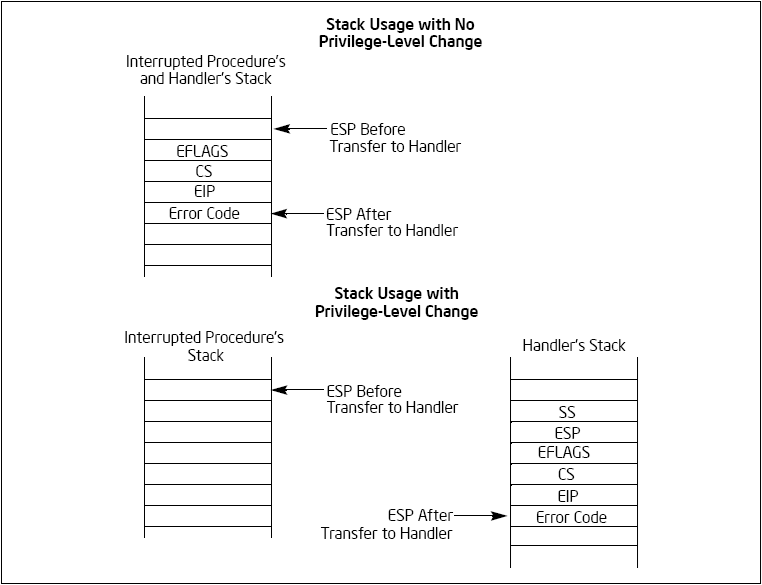
\includegraphics[scale=0.4]{picture/chapt7/interrupt_stack.png}
      \caption{中断发生时CPU保存的现场}
\end{figure}

\par CPU在发生中断的时候是按照上问所描述的过程执行的,那操作系统需要做什么呢?

\par 首先是实现中断处理函数。按照Intel的规定,0~19号中断属于CPU所有\footnote{这些由CPU自身产生的中断也被称之为异常。},而且\allowbreak
第20-31号中断也被Intel保留,所以从32~255号才属于用户自定义中断。虽说是"用户自定义",其实在x86上有些中断按照习惯还是给予了固定\allowbreak
的设备。比如32号是timer中断,33号是键盘中断等等。

\par 中断处理函数怎么实现呢?直接可以进行相关的逻辑处理吗?当然不行了。CPU在中断产生时自动保存了部分的执行现场,但是依旧有很多\allowbreak
寄存器需要我们自己去保护和恢复,下面是CPU保护的寄存器和剩余需要保护的寄存器一起定义的结构体。

\begin{lstlisting}[language = C, caption = include/idt.h]
// 寄存器类型
typedef
struct pt_regs_t {
	uint32_t ds; 		// 用于保存用户的数据段描述符
	uint32_t edi; 		// 从 edi 到 eax 由 pusha 指令压入
	uint32_t esi; 
	uint32_t ebp;
	uint32_t esp;
	uint32_t ebx;
	uint32_t edx;
	uint32_t ecx;
	uint32_t eax;
	uint32_t int_no; 	// 中断号
	uint32_t err_code;  	// 错误代码(有中断错误代码的中断会由CPU压入)
	uint32_t eip; 		// 以下由处理器自动压入
	uint32_t cs; 		
	uint32_t eflags;
	uint32_t useresp;
	uint32_t ss;
} pt_regs;

// 定义中断处理函数指针
typedef void (*interrupt_handler_t)(pt_regs *);

// 注册一个中断处理函数
void register_interrupt_handler(uint8_t n, interrupt_handler_t h);

// 调用中断处理函数
void isr_handler(pt_regs *regs);

// 声明中断处理函数 0-19 属于 CPU 的异常中断
// ISR:中断服务程序(interrupt service routine)
void isr0(); 		// 0 #DE 除 0 异常 
void isr1(); 		// 1 #DB 调试异常 
void isr2(); 		// 2 NMI 
void isr3(); 		// 3 BP 断点异常 
void isr4(); 		// 4 #OF 溢出 
void isr5(); 		// 5 #BR 对数组的引用超出边界 
void isr6(); 		// 6 #UD 无效或未定义的操作码 
void isr7(); 		// 7 #NM 设备不可用(无数学协处理器) 
void isr8(); 		// 8 #DF 双重故障(有错误代码) 
void isr9(); 		// 9 协处理器跨段操作 
void isr10(); 		// 10 #TS 无效TSS(有错误代码) 
void isr11(); 		// 11 #NP 段不存在(有错误代码) 
void isr12(); 		// 12 #SS 栈错误(有错误代码) 
void isr13(); 		// 13 #GP 常规保护(有错误代码) 
void isr14(); 		// 14 #PF 页故障(有错误代码) 
void isr15(); 		// 15 CPU 保留 
void isr16(); 		// 16 #MF 浮点处理单元错误 
void isr17(); 		// 17 #AC 对齐检查 
void isr18(); 		// 18 #MC 机器检查 
void isr19(); 		// 19 #XM SIMD(单指令多数据)浮点异常

// 20-31 Intel 保留
void isr20();
void isr21();
void isr22();
void isr23();
void isr24();
void isr25();
void isr26();
void isr27();
void isr28();
void isr29();
void isr30();
void isr31();

// 32~255 用户自定义异常
void isr255();
\end{lstlisting}

\par 一个很现实的问题是:所有的中断处理函数中,除了CPU本身保护的现场外,其它寄存器的保存和恢复过程都是一样的。所以,\allowbreak
如果在每个中断处理函数中都实现一次显然冗余而且易错。所以我们很自然把原本的中断处理函数逻辑上拆解为三部分,第一部分是\allowbreak
一致的现场保护操作;第二部分是每个中断特有的处理逻辑;第三部分又是一致的现场恢复。

\par 实际上我们把每个中断处理函数拆解为四段,在四个函数里实现。具体的实现如下:

\begin{lstlisting}[language = {[x86masm]Assembler}, caption = gdt/gdt\_s.s]
; 定义两个构造中断处理函数的宏(有的中断有错误代码,有的没有)
; 用于没有错误代码的中断
%macro ISR_NOERRCODE 1
[GLOBAL isr%1]
isr%1:
	cli                  ; 首先关闭中断
	push 0               ; push 无效的中断错误代码
	push %1              ; push 中断号
	jmp isr_common_stub
%endmacro

; 用于有错误代码的中断
%macro ISR_ERRCODE 1
[GLOBAL isr%1]
isr%1:
	cli                  ; 关闭中断
	push %1              ; push 中断号
	jmp isr_common_stub
%endmacro

; 定义中断处理函数
ISR_NOERRCODE  0 	; 0 #DE 除 0 异常
ISR_NOERRCODE  1 	; 1 #DB 调试异常
ISR_NOERRCODE  2 	; 2 NMI
ISR_NOERRCODE  3 	; 3 BP 断点异常 
ISR_NOERRCODE  4 	; 4 #OF 溢出 
ISR_NOERRCODE  5 	; 5 #BR 对数组的引用超出边界 
ISR_NOERRCODE  6 	; 6 #UD 无效或未定义的操作码 
ISR_NOERRCODE  7 	; 7 #NM 设备不可用(无数学协处理器) 
ISR_ERRCODE    8 	; 8 #DF 双重故障(有错误代码) 
ISR_NOERRCODE  9 	; 9 协处理器跨段操作
ISR_ERRCODE   10 	; 10 #TS 无效TSS(有错误代码) 
ISR_ERRCODE   11 	; 11 #NP 段不存在(有错误代码) 
ISR_ERRCODE   12 	; 12 #SS 栈错误(有错误代码) 
ISR_ERRCODE   13 	; 13 #GP 常规保护(有错误代码) 
ISR_ERRCODE   14 	; 14 #PF 页故障(有错误代码) 
ISR_NOERRCODE 15 	; 15 CPU 保留 
ISR_NOERRCODE 16 	; 16 #MF 浮点处理单元错误 
ISR_ERRCODE   17 	; 17 #AC 对齐检查 
ISR_NOERRCODE 18 	; 18 #MC 机器检查 
ISR_NOERRCODE 19 	; 19 #XM SIMD(单指令多数据)浮点异常

; 20~31 Intel 保留
ISR_NOERRCODE 20
ISR_NOERRCODE 21
ISR_NOERRCODE 22
ISR_NOERRCODE 23
ISR_NOERRCODE 24
ISR_NOERRCODE 25
ISR_NOERRCODE 26
ISR_NOERRCODE 27
ISR_NOERRCODE 28
ISR_NOERRCODE 29
ISR_NOERRCODE 30
ISR_NOERRCODE 31
; 32~255 用户自定义
ISR_NOERRCODE 255
\end{lstlisting}

\par 函数执行的开始位置我们自行向栈里压入中断的号码,这是为了识别出中断号码。上面的代码用到了NASM的宏汇编,因为指令结构\allowbreak
是相同的,所以我们可以用宏汇编来生成代码。如果大家对这里有疑问的话,可以参考NASM手册或者直接对生成的内核文件反汇编查看相\allowbreak
关函数的实现。另外还有一点需要说明的是,因为有的中断处理函数会自动压入错误号,而有的不会,这样给我们的清栈造成了麻烦。\allowbreak
所以我们在不会压入错误号的中断的处理函数里手动压入0作为占位,这样方便我们在清理的时候不用分类处理。

\par 以上是中断处理函数的最前一部分,接下来是所有中断处理函数共有的保护现场操作:
\begin{lstlisting}[language = {[x86masm]Assembler}, caption = gdt/gdt\_s.s]
[GLOBAL isr_common_stub]
[EXTERN isr_handler]
; 中断服务程序
isr_common_stub:
	pusha                    ; Pushes edi, esi, ebp, esp, ebx, edx, ecx, eax
	mov ax, ds
	push eax                ; 保存数据段描述符
	
	mov ax, 0x10            ; 加载内核数据段描述符表
	mov ds, ax
	mov es, ax
	mov fs, ax
	mov gs, ax
	mov ss, ax
	
	push esp		; 此时的 esp 寄存器的值等价于 pt_regs 结构体的指针
	call isr_handler        ; 在 C 语言代码里
	add esp, 4 		; 清除压入的参数
	
	pop ebx                 ; 恢复原来的数据段描述符
	mov ds, bx
	mov es, bx
	mov fs, bx
	mov gs, bx
	mov ss, bx
	
	popa                     ; Pops edi, esi, ebp, esp, ebx, edx, ecx, eax
	add esp, 8               ; 清理栈里的 error code 和 ISR
	iret
.end:
\end{lstlisting}

\par 这里声明了一个外部函数idt\_handler,它的实现如下:
\begin{lstlisting}[language = C, caption = gdt/gdt.c]
// 调用中断处理函数
void isr_handler(pt_regs *regs)
{
	if (interrupt_handlers[regs->int_no]) {
	      interrupt_handlers[regs->int_no](regs);
	} else {
		printk_color(rc_black, rc_blue, "Unhandled interrupt: %d\n", regs->int_no);
	}
}
\end{lstlisting}

\par 从上面的代码中我们看到,事实上具体的中断处理函数的原型都是 void (pt\_regs *),它们被统一组织放置在了全局的函数指针\allowbreak
数组interrupt\_handers里面。idt\_hanlder函数如判断这个中断函数是否注册,如果注册了会执行该函数,否则打印出Unhandled interrupt和\allowbreak
中断号码。

\par 最后是中断描述符表的创建和和加载函数:
\begin{lstlisting}[language = C, caption = gdt/gdt.c]
#include "common.h"
#include "string.h"
#include "debug.h"
#include "idt.h"

// 中断描述符表
idt_entry_t idt_entries[256];

// IDTR
idt_ptr_t idt_ptr;

// 中断处理函数的指针数组
interrupt_handler_t interrupt_handlers[256];

// 设置中断描述符
static void idt_set_gate(uint8_t num, uint32_t base, uint16_t sel, uint8_t flags);

// 声明加载 IDTR 的函数
extern void idt_flush(uint32_t);

// 初始化中断描述符表
void init_idt()
{	
	bzero((uint8_t *)&interrupt_handlers, sizeof(interrupt_handler_t) * 256);
	
	idt_ptr.limit = sizeof(idt_entry_t) * 256 - 1;
	idt_ptr.base  = (uint32_t)&idt_entries;
	
	bzero((uint8_t *)&idt_entries, sizeof(idt_entry_t) * 256);

	// 0-32:  用于 CPU 的中断处理
	idt_set_gate( 0, (uint32_t)isr0,  0x08, 0x8E);
	idt_set_gate( 1, (uint32_t)isr1,  0x08, 0x8E);
	idt_set_gate( 2, (uint32_t)isr2,  0x08, 0x8E);
	idt_set_gate( 3, (uint32_t)isr3,  0x08, 0x8E);
	idt_set_gate( 4, (uint32_t)isr4,  0x08, 0x8E);
	idt_set_gate( 5, (uint32_t)isr5,  0x08, 0x8E);
	idt_set_gate( 6, (uint32_t)isr6,  0x08, 0x8E);
	idt_set_gate( 7, (uint32_t)isr7,  0x08, 0x8E);
	idt_set_gate( 8, (uint32_t)isr8,  0x08, 0x8E);
	idt_set_gate( 9, (uint32_t)isr9,  0x08, 0x8E);
	idt_set_gate(10, (uint32_t)isr10, 0x08, 0x8E);
	idt_set_gate(11, (uint32_t)isr11, 0x08, 0x8E);
	idt_set_gate(12, (uint32_t)isr12, 0x08, 0x8E);
	idt_set_gate(13, (uint32_t)isr13, 0x08, 0x8E);
	idt_set_gate(14, (uint32_t)isr14, 0x08, 0x8E);
	idt_set_gate(15, (uint32_t)isr15, 0x08, 0x8E);
	idt_set_gate(16, (uint32_t)isr16, 0x08, 0x8E);
	idt_set_gate(17, (uint32_t)isr17, 0x08, 0x8E);
	idt_set_gate(18, (uint32_t)isr18, 0x08, 0x8E);
	idt_set_gate(19, (uint32_t)isr19, 0x08, 0x8E);
	idt_set_gate(20, (uint32_t)isr20, 0x08, 0x8E);
	idt_set_gate(21, (uint32_t)isr21, 0x08, 0x8E);
	idt_set_gate(22, (uint32_t)isr22, 0x08, 0x8E);
	idt_set_gate(23, (uint32_t)isr23, 0x08, 0x8E);
	idt_set_gate(24, (uint32_t)isr24, 0x08, 0x8E);
	idt_set_gate(25, (uint32_t)isr25, 0x08, 0x8E);
	idt_set_gate(26, (uint32_t)isr26, 0x08, 0x8E);
	idt_set_gate(27, (uint32_t)isr27, 0x08, 0x8E);
	idt_set_gate(28, (uint32_t)isr28, 0x08, 0x8E);
	idt_set_gate(29, (uint32_t)isr29, 0x08, 0x8E);
	idt_set_gate(30, (uint32_t)isr30, 0x08, 0x8E);
	idt_set_gate(31, (uint32_t)isr31, 0x08, 0x8E);

	// 255 将来用于实现系统调用
	idt_set_gate(255, (uint32_t)isr255, 0x08, 0x8E);

	// 更新设置中断描述符表
	idt_flush((uint32_t)&idt_ptr);
}

// 设置中断描述符
static void idt_set_gate(uint8_t num, uint32_t base, uint16_t sel, uint8_t flags)
{
	idt_entries[num].base_lo = base & 0xFFFF;
	idt_entries[num].base_hi = (base >> 16) & 0xFFFF;

	idt_entries[num].sel     = sel;
	idt_entries[num].always0 = 0;

	// 先留下 0x60 这个魔数,以后实现用户态时候
	// 这个与运算可以设置中断门的特权级别为 3
	idt_entries[num].flags = flags;  // | 0x60
}
\end{lstlisting}

\par 加载中断描述符表的函数很简单:
\begin{lstlisting}[language = {[x86masm]Assembler}, caption = gdt/gdt\_s.s]
[GLOBAL idt_flush]
idt_flush:
	mov eax, [esp+4]  ; 参数存入 eax 寄存器
	lidt [eax]        ; 加载到 IDTR
	ret
.end:
\end{lstlisting}

\par 整理好上面的代码,修改入口函数测试一下中断吧。入口代码修改如下:
\begin{lstlisting}[language = C, caption = init/entry.c]
#include "console.h"
#include "debug.h"
#include "gdt.h"
#include "idt.h"

int kern_entry()
{
	init_debug();
	init_gdt();
	init_idt();

	console_clear();
	printk_color(rc_black, rc_green, "Hello, OS kernel!\n");

	asm volatile ("int $0x3");
	asm volatile ("int $0x4");

	return 0;
}
\end{lstlisting}

\par 编译运行,我们得要了正确的结果:\footnote{当然了,我们没有注册具体的处理函数,所以就打印默认的信息了。}
\begin{figure}[ht]
      \centering
      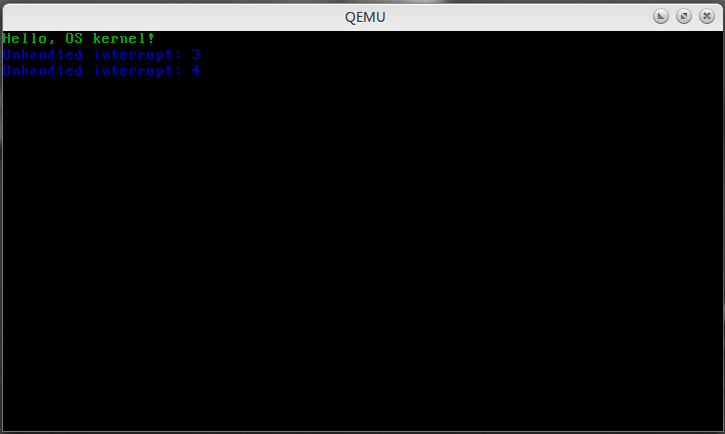
\includegraphics[scale=0.5]{picture/chapt7/interrupt_view.png}
      \caption{中断处理函数的测试}
\end{figure}
